\section{Datenanalyse}

Um Aussagen über Zusammenhänge zwischen zwei Größen zu treffen, wurden bis jetzt immer nur die Geradengleichungen der Regressionsgeraden benutzt.
Das Problem dabei ist, dass wir nur einen Mittelwert haben, aber nicht wissen, wie stark unsere Werte streuen, also wie präzise sie sind.
Weiter kann man mit der Datenanalyse noch bestimmen, wie sauber gearbeitet wurde und ob das verwendete Verfahren für das Problem gute Messergebnisse
liefert. \\
Um die Streuung der Daten zu berechnen verwendet man die Residuenanalyse. Dabei wird die errechnete Geradengleichung genommen, welche durch den
Datensatz läuft und berechnet dann die mittlere Abweichung der einzelnen Datenpunkte zu der Geraden. \\
Mit der Residuenanalyse werden die Datensätze zu Abbildung 2 und 4 untersucht.

\begin{enumerate}
    \item Bestimmung der Geradengleichung
    % Table generated by Excel2LaTeX from sheet 'Vergleich'
\begin{table}[H]
  \centering
  \caption{Gradengleichungen}
    \begin{tabular}{lcc}
    \toprule
          & \multicolumn{1}{l}{\boldmath{}\textbf{25$^\circ$C}\unboldmath{}} & \multicolumn{1}{l}{\boldmath{}\textbf{40$^\circ$C}\unboldmath{}} \\
    \midrule
    \textbf{Steigung} & -0,5  & -0,5 \\
    \textbf{Achsenabschnitt} & 0,983 & 0,9937 \\
    \bottomrule
    \end{tabular}%
  \label{tab:addlabel}%
\end{table}%

    \item Residuen Berechnen über:
    % Table generated by Excel2LaTeX from sheet 'Vergleich'
\begin{table}[H]
  \centering
  \caption{Berechnung der Residuen bei 25$^\circ$C}
    \begin{tabular}{cccc}
    \toprule
    \multicolumn{1}{l}{\boldmath{}\textbf{$x_i$ [mmol/kg]}\unboldmath{}} & \multicolumn{1}{l}{\boldmath{}\textbf{$y_i$}\unboldmath{}} & \multicolumn{1}{l}{\boldmath{}\textbf{$\hat{y}_i$}\unboldmath{}} & \multicolumn{1}{l}{\boldmath{}\textbf{$y_i - \hat{y}_i$}\unboldmath{}} \\
    \midrule
    50,012 & 1,644 & 1,633 & 0,011 \\
    25,006 & 1,795 & 1,784 & 0,011 \\
    15,058 & 1,905 & 1,894 & 0,011 \\
    10,062 & 1,992 & 1,982 & 0,011 \\
    6,048 & 2,103 & 2,092 & 0,011 \\
    5,009 & 2,144 & 2,133 & 0,011 \\
    1,004 & 2,493 & 2,482 & 0,011 \\
    0,997 & 2,494 & 2,484 & 0,011 \\
    0,804 & 2,541 & 2,530 & 0,011 \\
    0,607 & 2,602 & 2,591 & 0,011 \\
    0,505 & 2,642 & 2,631 & 0,011 \\
    0,407 & 2,689 & 2,678 & 0,011 \\
    0,301 & 2,755 & 2,744 & 0,011 \\
    0,200 & 2,843 & 2,832 & 0,011 \\
    0,101 & 2,992 & 2,981 & 0,011 \\
    \bottomrule
    \end{tabular}%
  \label{tab:addlabel}%
\end{table}%

    \item Standardabweichung der Residuen bestimmen:
        \begin{itemize}
            \item Die Standardabweichung bei 25$^\circ$C ist $\sigma_{25} = \pm 1,636 \cdot 10^{-16}$
            \item Die Standardabweichung bei 40$^\circ$C ist $\sigma_{40} = \pm 2,1992 \cdot 10^{-16}$
        \end{itemize}
\end{enumerate} 

Bei diesen extrem kleinen Standardabweichungen kann davon Aussagen werden, dass keine Fehler bei der Durchführung aufgetreten sind und es 
eigentlich keinen Sinn macht die Ergebnisse mit Standardabweichung anzugeben. 
Wenn man den Graphen von dem Debye-Radius gegen die logarithmierte Konzentration mit Standardabweichung zeichnet, sieht man nur einen Datensatz,
da die Streuung so klein ist.

\begin{figure}[H]
    \centering
    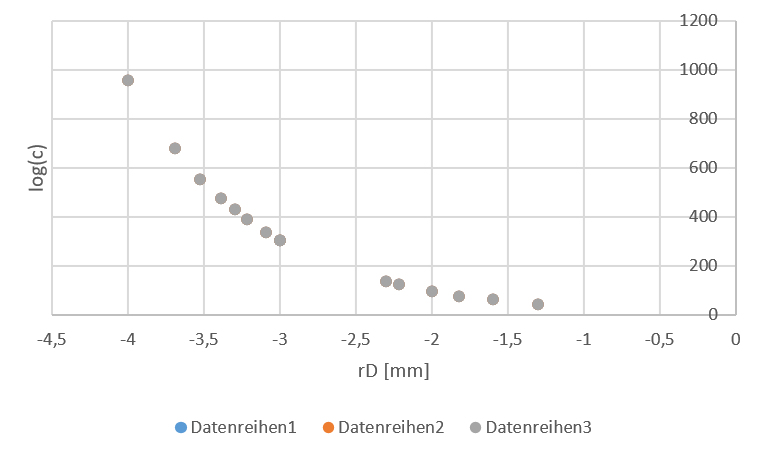
\includegraphics[scale=.7]{../src/img/graph3_25C.png}
\end{figure}

\begin{figure}[H]
    \centering
    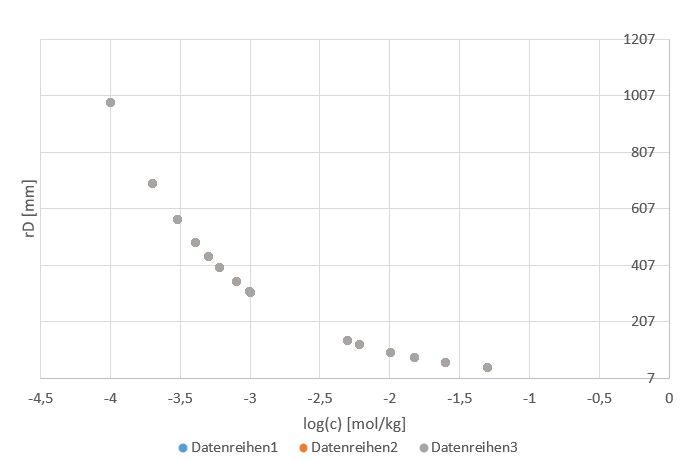
\includegraphics[scale=.7]{../src/img/graph3_40C.png}
\end{figure}


\subsection{Bestimmung der Unterschiede des Debye-Radius im Hinblick auf die Temperatur}

Um zu bestimmen, welchen Einfluss die Temperatur auf den Debye-Radius hat, teilt man die entsprechenden Werte der einen Temperatur durch die der
andern. Als nächstes kann dann noch der prozentuale Unterschied bestimmt werden, dafür wird von dem vorher berechneten Verhältnis 1 abgezogen und
dann mit 100 multipliziert.

% Table generated by Excel2LaTeX from sheet 'Vergleich'
\begin{table}[H]
  \centering
  \caption{Unterschied des Debye-Radiuses bei verschiedenen Temperaturen}
    \begin{tabular}{ccc}
    \toprule
    \multicolumn{1}{c}{\textbf{lg(konz)}} & \multicolumn{1}{p{6.785em}}{\textbf{\qquad X = \newline{}rD(40$^\circ$C/25$^\circ$C)}} & \multicolumn{1}{c}{\textbf{(X-1.0)*100}} \\
    \midrule
    -1,30092578 & 0,975663369 & -2,43366306 \\
    -1,60195577 & 0,975663369 & -2,43366306 \\
    -1,82221977 & 0,975663369 & -2,43366306 \\
    -1,99730297 & 0,975663369 & -2,43366306 \\
    -2,21841747 & 0,975663369 & -2,43366306 \\
    -2,30023174 & 0,975663369 & -2,43366306 \\
    -2,99826542 & 0,975663369 & -2,43366306 \\
    -3,00130224 & 0,975663369 & -2,43366306 \\
    -3,09467784 & 0,975663369 & -2,43366306 \\
    -3,21698447 & 0,975663369 & -2,43366306 \\
    -3,29670261 & 0,975663369 & -2,43366306 \\
    -3,39031898 & 0,975663369 & -2,43366306 \\
    -3,52204004 & 0,975663369 & -2,43366306 \\
    -3,69792895 & 0,975663369 & -2,43366306 \\
    -3,99611731 & 0,975663369 & -2,43366306 \\
    \bottomrule
    \end{tabular}%
  \label{tab:addlabel}%
\end{table}%




Wie man aus der Tabelle entnehmen kann, verändert sich der Anstieg der Werte so gut wie nicht. Dies ist aber auch zu
erwarten, da die Steigungen der Regressionsgeraden gleich sind ($m = -0.5$).

\begin{figure}[H]
    \centering
    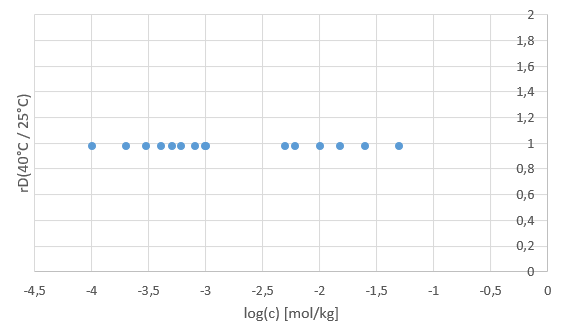
\includegraphics[scale=.7]{../src/img/graph1_vergleich.png}
    \caption{Debye-Radius im Hinblick auf die Temperatur}
\end{figure}

Es lässt sich kein Zusammenhang zwischen der Temperatur und dem Anstieg des Debye-Radius mit der Konzentration zeigen. Obwohl anzunehmen wäre
das der Debye-Radius mit erniedrigung der Temperatur umso schneller wächst, je geringer Temperatur ist. Wenn man also noch den prozentualen
Verlauf visualisiert, sollte man einen  positiven linearen Zusammenhang erkennen können.

\begin{figure}[H]
    \centering
    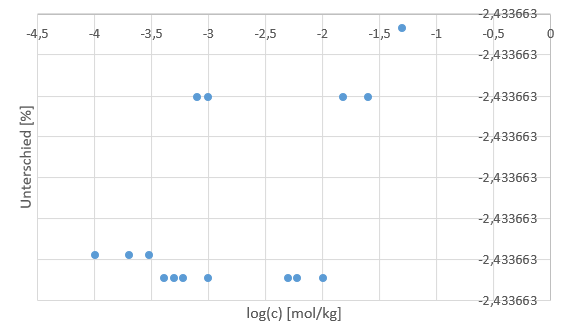
\includegraphics[scale=.7]{../src/img/graph2_vergleich.png}
    \caption{Debye-Radius im Hinblick auf die Temperatur}
\end{figure}

Wie man der Datenverteilung entnehmen kann ist dies nicht der Fall, es fällt aber auf, dass die y-Achse sich nicht ändert, sie zeigt immer den 
gleichen Wert an. Möglicherweise sind die Werte zu klein und Excel kann sie nicht mehr darstellen. Da hier dem ersten Anschein nach etwas falsch ist
werde ich versuche die Methodik zu überprüfen indem ich die gleiche Datenanalyse für die Werte der Dissoziation durchexerziere.

\subsection{Datenanalyse für die Graphiken der Dissoziation}

\subsubsection{Auswertung der Messwerte bei 25$^\circ$C}

Für die Berechnung der Residuen erhält man folgende Werte:

% Table generated by Excel2LaTeX from sheet 'Tabelle3'
\begin{table}[H]
  \centering
  \caption{Residuenanalyse bei 25$^\circ$C}
    \begin{tabular}{cccc}
    \toprule
    \multicolumn{1}{l}{\boldmath{}\textbf{$x_i$ [mmol/kg]}\unboldmath{}} & \multicolumn{1}{l}{\boldmath{}\textbf{$y_i$}\unboldmath{}} & \multicolumn{1}{l}{\boldmath{}\textbf{$\hat{y}_i$}\unboldmath{}} & \multicolumn{1}{l}{\boldmath{}\textbf{$y_i - \hat{y}_i$}\unboldmath{}} \\
    \midrule
    -1,301 & 0,271 & 0,310 & -0,040 \\
    -1,602 & 0,462 & 0,447 & 0,015 \\
    -1,822 & 0,572 & 0,547 & 0,025 \\
    -1,997 & 0,617 & 0,627 & -0,009 \\
    -2,218 & 0,718 & 0,727 & -0,009 \\
    -2,300 & 0,770 & 0,764 & 0,006 \\
    -2,998 & 1,088 & 1,081 & 0,007 \\
    -3,001 & 1,091 & 1,082 & 0,009 \\
    -3,095 & 1,135 & 1,125 & 0,010 \\
    -3,217 & 1,187 & 1,180 & 0,007 \\
    -3,297 & 1,227 & 1,216 & 0,010 \\
    -3,390 & 1,260 & 1,259 & 0,001 \\
    -3,522 & 1,312 & 1,319 & -0,007 \\
    -3,698 & 1,408 & 1,398 & 0,009 \\
    -3,996 & 1,496 & 1,534 & -0,038 \\
    \bottomrule
    \end{tabular}%
  \label{tab:addlabel}%
\end{table}%


Daraus ergibt sich folgende Graphik:

\begin{figure}[H]
    \centering
    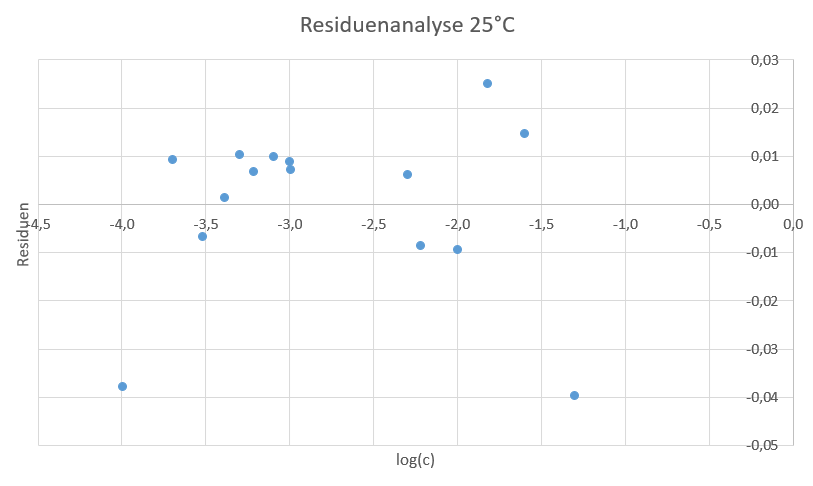
\includegraphics[scale=.7]{../src/img/residuen_25C.png}
    \caption{Auswertung der Messwerte bei 25$^\circ$C}
\end{figure}

Die Standardabweichung beträgt $\sigma = \pm 0.018$. Somit ist die Geradengleichung gegeben durch:

\begin{align*}
    y = -0.4539 x - 0.28 \pm 0.018
\end{align*}

\subsubsection{Auswertung der Messwerte bei 40$^\circ$C}

Für die Residuen ergeben sich diesmal: 

% Table generated by Excel2LaTeX from sheet 'Tabelle3'
\begin{table}[H]
  \centering
  \caption{Residuenanalyse bei 40$^\circ$C}
    \begin{tabular}{cccc}
    \toprule
    \multicolumn{1}{l}{\boldmath{}\textbf{$x_i$ [mmol/kg]}\unboldmath{}} & \multicolumn{1}{l}{\boldmath{}\textbf{$y_i$}\unboldmath{}} & \multicolumn{1}{l}{\boldmath{}\textbf{$\hat{y}_i$}\unboldmath{}} & \multicolumn{1}{l}{\boldmath{}\textbf{$y_i - \hat{y}_i$}\unboldmath{}} \\
    \midrule
    -1,30093 & 0,24093 & 0,26706 & -0,02614 \\
    -1,60196 & 0,40196 & 0,40427 & -0,00232 \\
    -1,82222 & 0,50222 & 0,50467 & -0,00245 \\
    -1,99730 & 0,58730 & 0,58447 & 0,00283 \\
    -2,21842 & 0,68842 & 0,68525 & 0,00316 \\
    -2,30023 & 0,73023 & 0,72255 & 0,00769 \\
    -2,99827 & 1,05827 & 1,04071 & 0,01756 \\
    -3,00130 & 1,06130 & 1,04209 & 0,01921 \\
    -3,09468 & 1,09468 & 1,08465 & 0,01002 \\
    -3,21698 & 1,14698 & 1,14040 & 0,00658 \\
    -3,29670 & 1,18670 & 1,17674 & 0,00997 \\
    -3,39032 & 1,23032 & 1,21941 & 0,01091 \\
    -3,52204 & 1,26204 & 1,27945 & -0,01741 \\
    -3,69793 & 1,35793 & 1,35962 & -0,00169 \\
    -3,99612 & 1,45612 & 1,49553 & -0,03941 \\
    \bottomrule
    \end{tabular}%
  \label{tab:addlabel}%
\end{table}%


Und daraus ergibt sich folgende Graphik 

\begin{figure}[H]
    \centering
    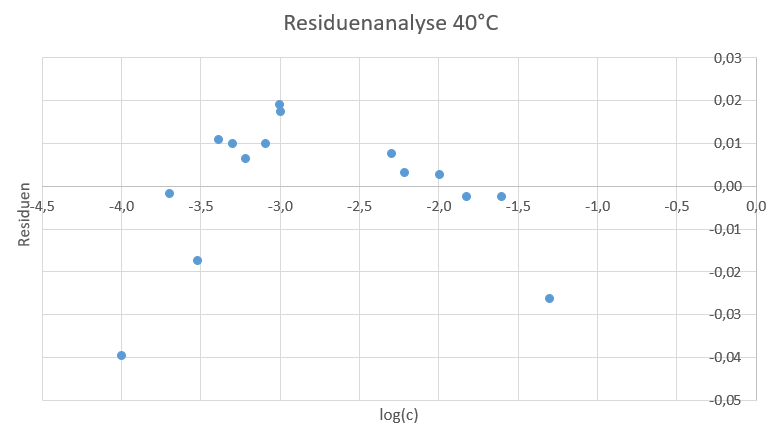
\includegraphics[scale=.7]{../src/img/residuen_40C.png}
    \caption{Auswertung der Messwerte bei 40$^\circ$C}
\end{figure}

Die Standardabweichung beträgt $\sigma = \pm 0.016$. Somit ist die Geradengleichung gegeben durch:

\begin{align*}
    y = -0.4558 x - 0.32 \pm 0.016
\end{align*}


\subsubsection{Vergleich der Dissoziationen bei verschiedenen Temperaturen}

Wie bei dem Vergleich der Debye-Radien wird auch hier der Quotient und das daraus bestimmte prozentuelle Verhältnis hinsichtlich der Temperatur untersucht. 
Berechnet wurde hiefür folgendes:

% Table generated by Excel2LaTeX from sheet 'Tabelle3'
\begin{table}[H]
  \centering
  \caption{Temperaturvergleich}
    \begin{tabular}{ccc}
    \toprule
    \multicolumn{1}{c}{\textbf{lg(konz)}} & {\boldmath{}\textbf{\qquad X =  $\alpha (40^\circ C/25^\circ C)$}\unboldmath{}} & \multicolumn{1}{c}{\textbf{(X-1.0)*100}} \\
    \midrule
    -1,301 & 0,905 & -9,516 \\
    -1,602 & 0,906 & -9,397 \\
    -1,822 & 0,907 & -9,309 \\
    -1,997 & 0,908 & -9,240 \\
    -2,218 & 0,908 & -9,152 \\
    -2,300 & 0,909 & -9,120 \\
    -2,998 & 0,912 & -8,842 \\
    -3,001 & 0,912 & -8,840 \\
    -3,095 & 0,912 & -8,803 \\
    -3,217 & 0,912 & -8,754 \\
    -3,297 & 0,913 & -8,723 \\
    -3,390 & 0,913 & -8,685 \\
    -3,522 & 0,914 & -8,632 \\
    -3,698 & 0,914 & -8,562 \\
    -3,996 & 0,916 & -8,443 \\
    \bottomrule
    \end{tabular}%
  \label{tab:addlabel}%
\end{table}%


Aus diesen Werten lassen sich diese beiden Grafiken generieren.

\begin{figure}[H]
    \centering
    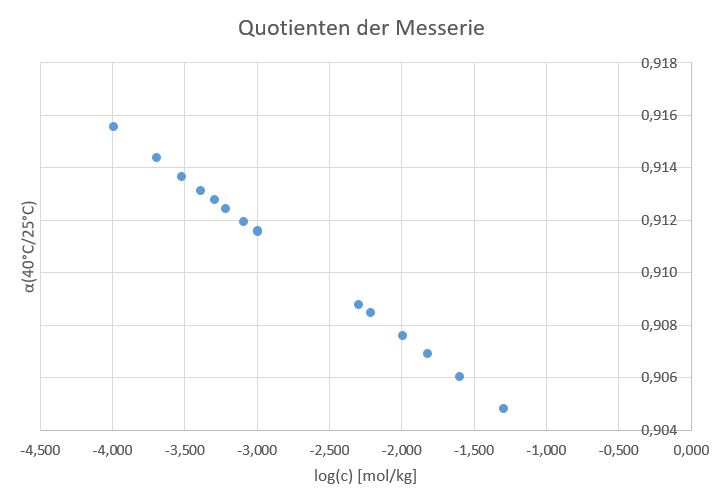
\includegraphics[scale=.7]{../src/img/alpha_quotient.png}
    \caption{Vergleich der Dissoziationen bei verschiedenen Temperaturen}
\end{figure}

\begin{figure}[H]
    \centering
    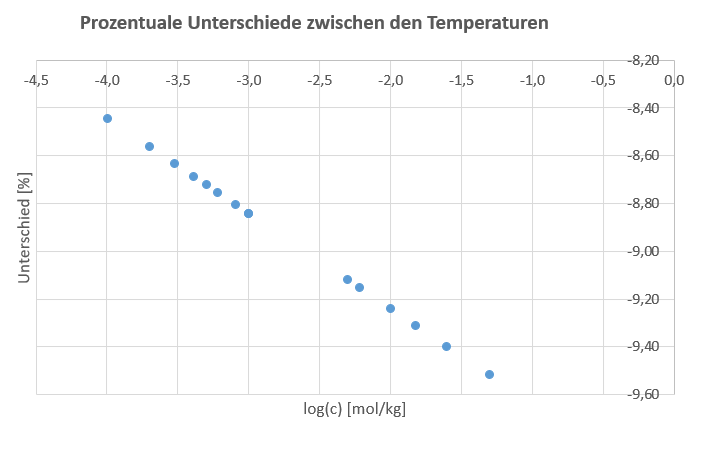
\includegraphics[scale=.7]{../src/img/alpha_prozent.png}
    \caption{Vergleich der Dissoziationen bei verschiedenen Temperaturen}
\end{figure}

Aus den Graphiken geht ein deutlicher linearer Zusammenhang hervor. Er zeigt, dass je kleiner die Konzentration ist, desto schneller steigt
die Dissoziation bei höheren Temperaturen. Desweiteren zeigt sich, dass die Berechnungen bei der Analyse des Debye-Radius korrekt waren und
es sich wahrscheinlich um einen Fehler inm excel-File handelt, welcher nicht gefunden wurde.   

